\chapter{Methode}\label{chap:m}
Die Methode dieser Untersuchung besteht darin, die in der Fragestellung
beschriebene künstliche Intelligenz (KI) zu entwickeln und dessen Leistung
auszuwerten. Die Diskussion dieser Resultate führt schlussendlich zu einer
Antwort auf die Fragestellung. Die Entwicklung der KI besteht aus zwei Teilen.
Der eine Teil umfasst die Definition der Kriterien, nach denen die Leistung der
KI evaluiert wird (siehe \doubleref{chap:m_eval}). Der andere Teil umfasst die
Entwicklung der KI (siehe \doubleref{chap:m_grund}), zusammen mit verschiedenen
Variationen davon (siehe \doubleref{chap:m_var}). Die Variationen haben jeweils
einen unterschiedlichen Fokus auf die definierten Kriterien. Die Auswertung
(siehe \doubleref{chap:m_auswert}) der Leistung der KI bezieht sich ebenfalls
auf die definierten Kriterien.

\section{Grundprogramm}\label{chap:m_grund} Die KI ist abhängig von den
Kriterien, die dessen Leistung definieren (siehe \doubleref{chap:m_eval}). Mit
anderen Worten trainiert die KI auf diese Kriterien. Das Ziel des
Grundprogrammes ist, die allgemeine Trainingsumgebung für die KI
bereitzustellen. Dieses Grundprogramm ist unabhängig von einem spezifischen
Kriterium und ermöglicht das Training auf ein beliebiges Kriterium.
Reinforcement Learning Modelle mit einer undefinierten Reward Function (siehe
\doubleref{sub:t_rl_func}) umfassen diese Eigenschaften. Das Grundprogramm ist
in Python unter der Verwendung des Keras Frameworks implementiert (siehe
\doubleref{chap:t_ml}). 

\subsection{Doodle-SDQ als Basis}\label{sub:m_grund_dood} Das Reinforcement
Learning Modell des Grundprogrammes basiert auf Doodle-SDQ (siehe
\doubleref{sub:t_ver_dood}). Von Doodle-SDQ ist das neuronale Netz, bezogen auf
die Form des Inputs, des Outputs und den Hidden Layers, grösstenteils
übernommen. Die relevanten Anpassungen zwischen Doodle-SDQ und dem Grundprogramm
dieser Arbeit sind nachfolgend erläutert.

Bei der Umgebung handelt es sich, wie bei Doodle-SDQ, um eine Zeichenfläche,
worauf sich der Agent bewegt. Das Grundprogramm wird auf das
Nachzeichnen von Ziffern trainiert. Die Ziffern stammen aus dem MNIST Datenset
(siehe \doubleref{chap:t_ml}) und haben somit eine Grösse von $28\times28$
Pixeln. Die Fläche, worauf sich der Agent bewegen   
kann, hat folglich auch eine Grösse von $28\times28$ Pixeln. Der Global Stream
(siehe \doubleref{sub:t_ver_dood}) des Inputs in das Neuronale Netz ändert sich
bis auf die neue Grösse der Bilder nicht. Die Pixel der Bilder, wie auch die
Zeichenfläche, nehmen den Wert von einem Bit an. Eine Null repräsentiert einen
schwarzen (nicht gezeichneten) Pixel an dieser Stelle im Bild und eine Eins
einen weissen (gezeichneten) Pixel. Die genaue Architektur des neuronalen Netzes
ist im Schema \autoref{fig:architecture} angegeben.

%Bild architecture
\begin{figure}[!ht]
  \centering
  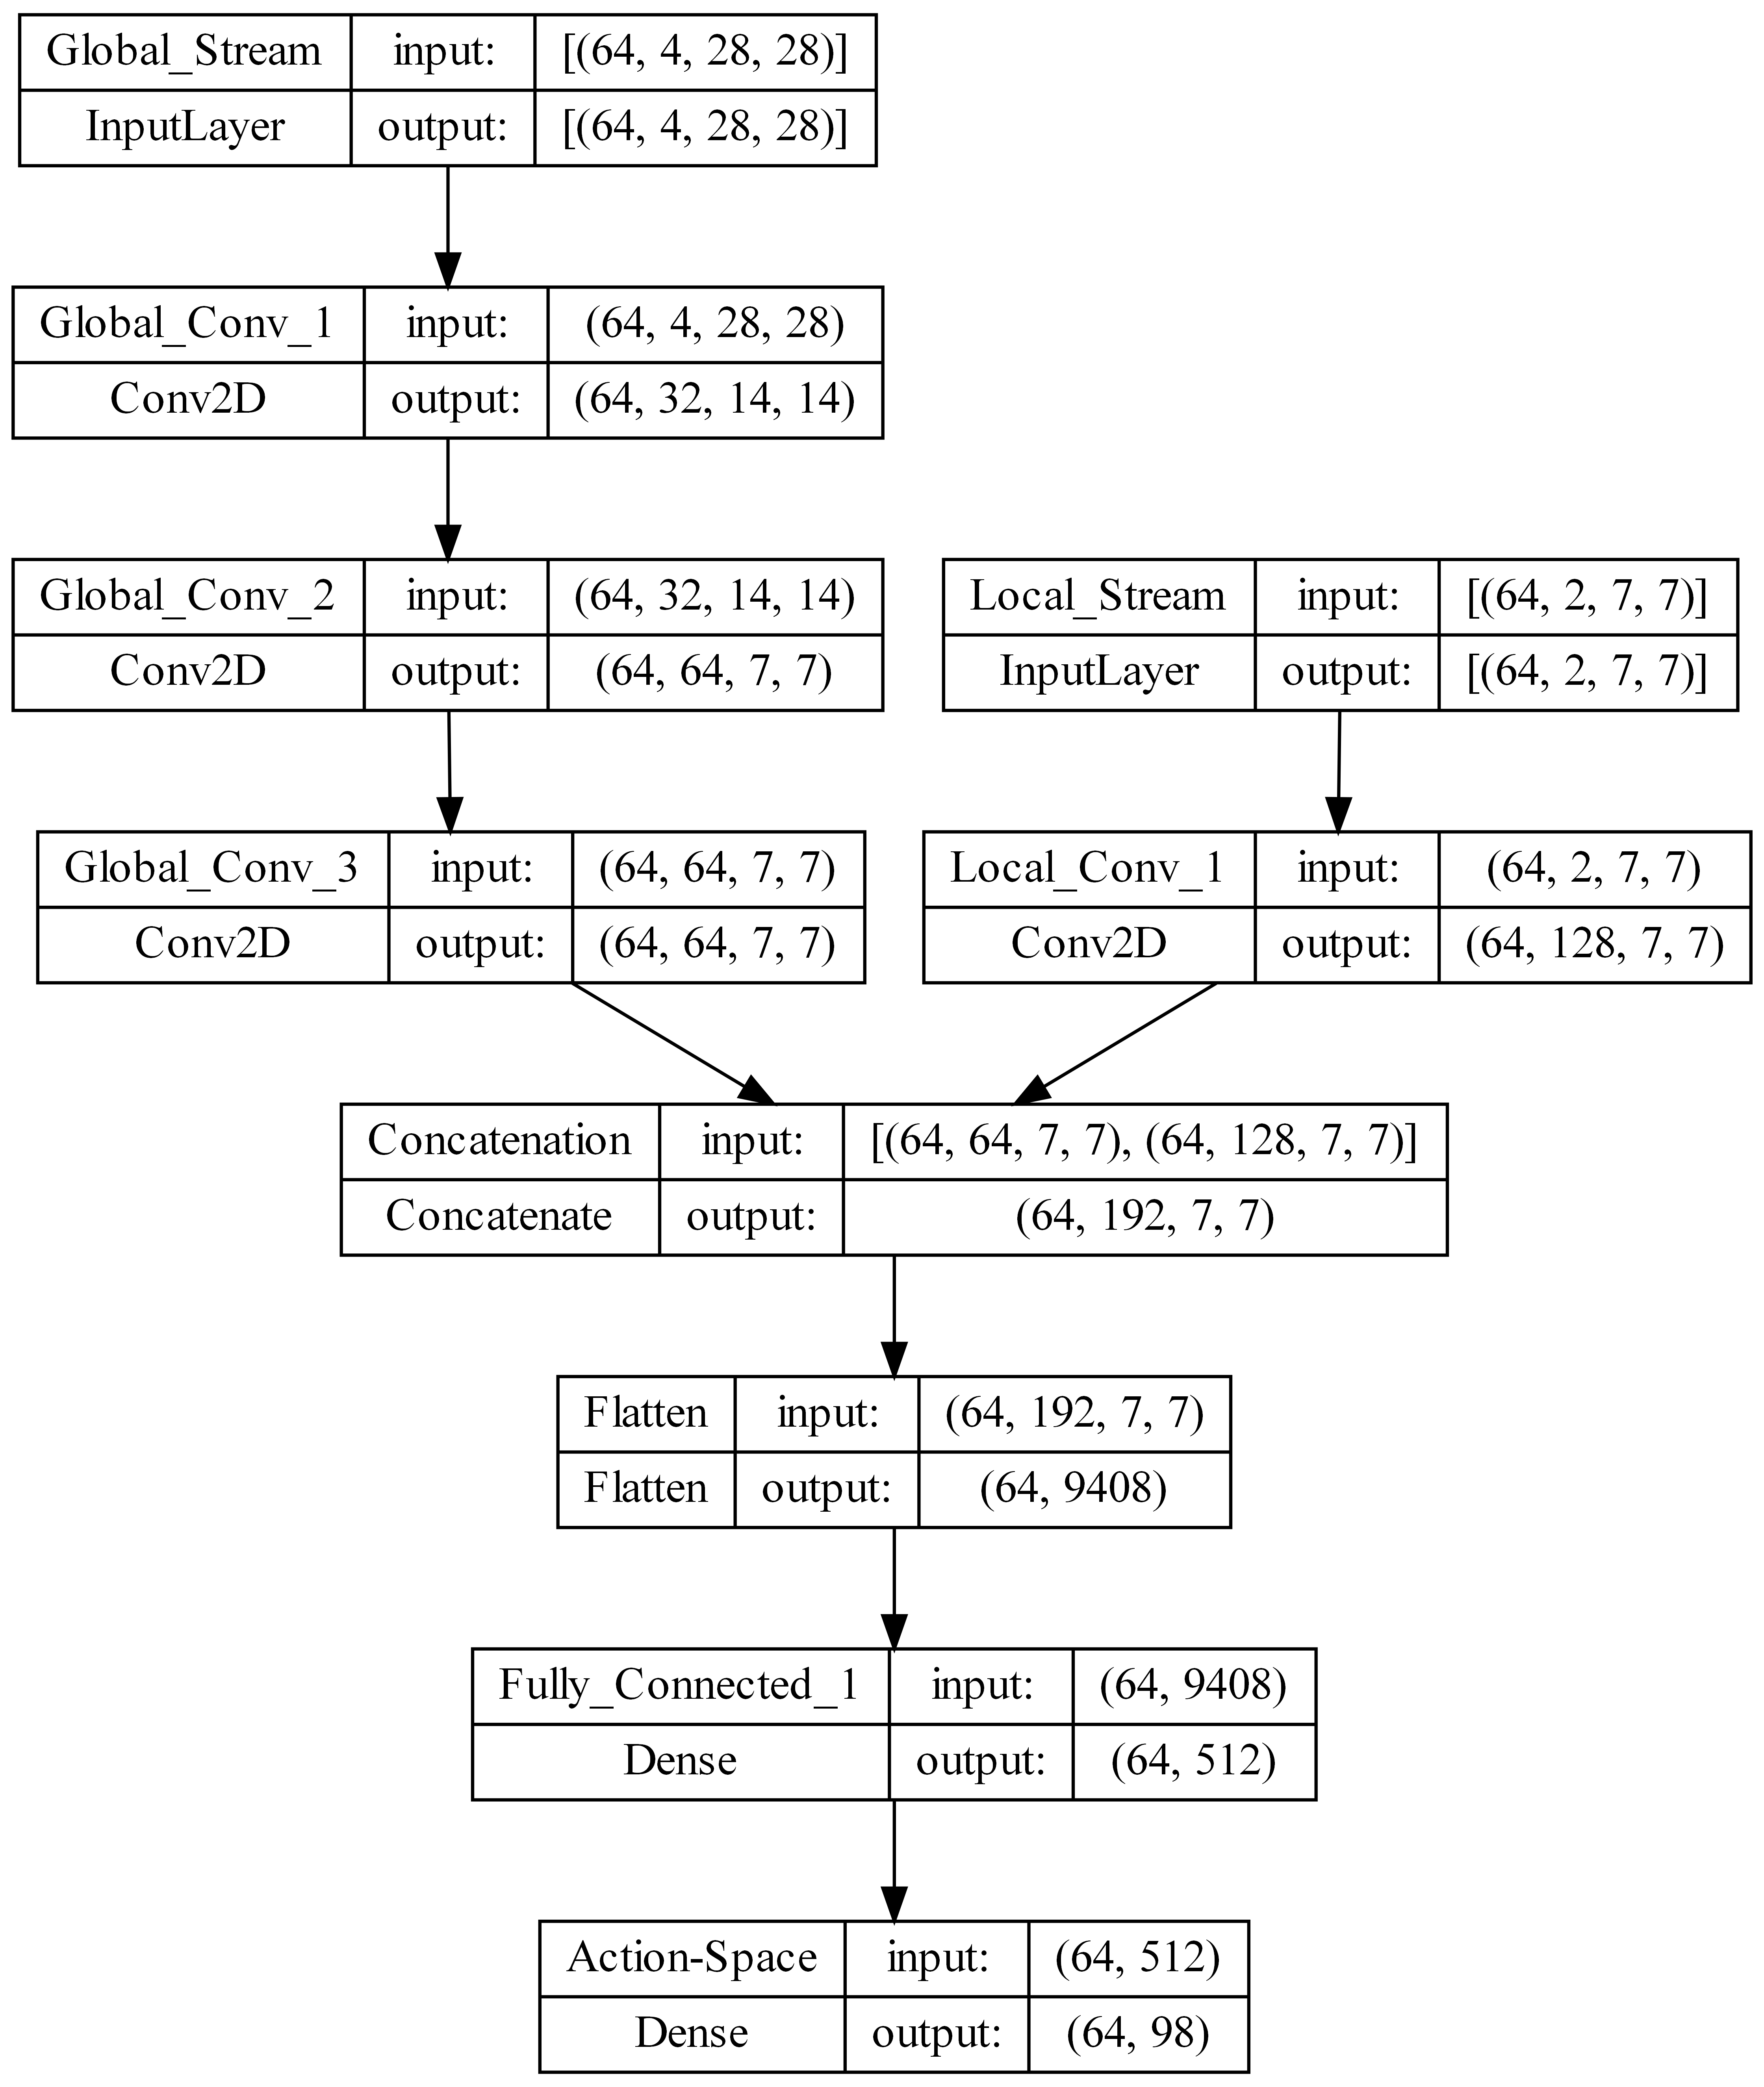
\includegraphics[width=\textwidth-2cm]{images/methode/architecture.png}
  \caption{Architektur des neuronalen Netzes im Grundprogramm (eigene Abbildung, mit Keras erstellt) Jeder Block repräsentiert einen Layer. Die Form des Inputs und des Outputs ist von jedem Layer angegeben}
  \label{fig:architecture}
\end{figure}

Der Local Stream und damit auch der Local image Patch schrumpfen von $11\times11$
Pixel auf $7\times7$ Pixel. Somit schrumpft gleichzeitig der Action-Space (siehe
\doubleref{sub:t_rl_func}) des Agenten von $2\cdot11\cdot11 = 242$ Actions auf
$2\cdot7\cdot7 = 98$ Actions. Das bedeutet für den Agent, dass er sich pro Step
um maximal drei Pixel von seiner Position wegbewegen kann. Diese Bewegung kann
der Agent entweder zeichnend oder nicht zeichnend ausführen (siehe
\autoref{fig:actionspace}).

%bild normal actionspace
\begin{figure}[!ht]
  \centering
  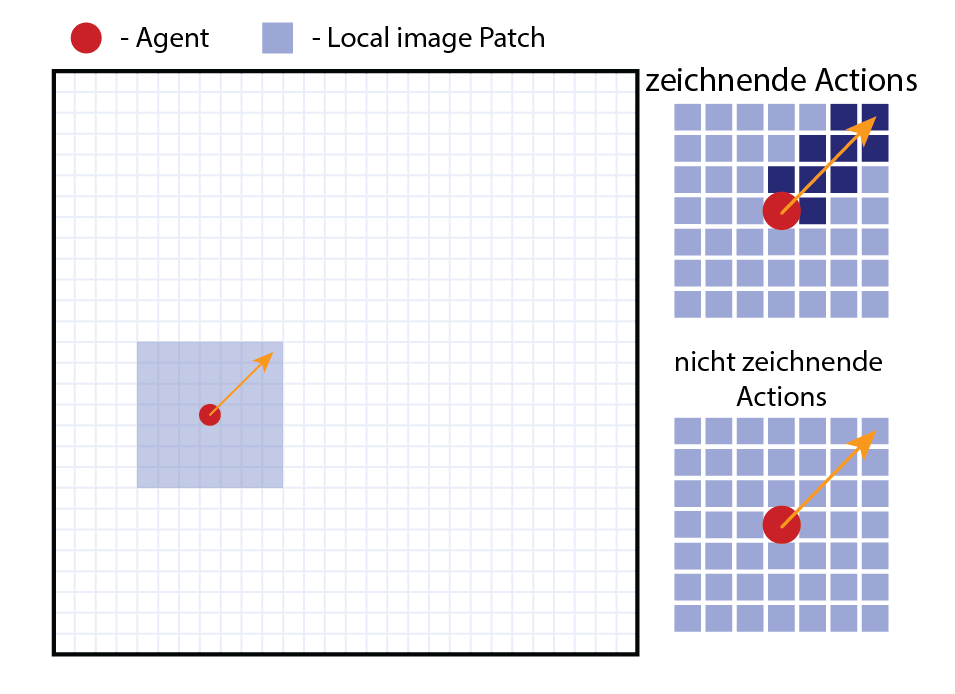
\includegraphics[width=\textwidth]{images/methode/actionspace.png}
  \caption{Action-Space im Grundprogramm}
  \label{fig:actionspace}
\end{figure}

Falls der Agent die Action zeichnend ausführt, zieht das Programm einen Strich
zwischen der alten und der neuen Position. Mit anderen Worten werden alle Pixel
der Zeichenfläche zwischen den beiden Positionen weiss. Der Strich hat eine
festgelegte Breite von $3$ Pixeln. Am Anfang jeder Episode, also mit jeder neuen
Ziffer, startet der Agent in einer zufälligen Position im nicht zeichnenden
Zustand. Am Anfang jeder Episode ist die Zeichenfläche leer, also vollkommen
Schwarz.

Actions des Agents, die ihn über die vorgegebene Zeichenfläche hinaus
positionieren würden, sind nicht zulässig. Diese Actions können vom Agent nicht
gewählt werden und ihr optimaler Q-Value (siehe \doubleref{sub:t_rl_func}) ist
in jedem Fall $0$. Das hat zur Folge, dass nach dem Training die allermeisten
unzulässigen Actions einen Q-Value nahe oder gleich $0$ haben. Das senkt die
Wahrscheinlichkeit, dass der Agent versucht, eine unzulässige Action
auszuführen.

\subsection{Präparierung der Daten und Optimierung}\label{sub:m_grund_data}
Die Trainingsdaten bestehen aus $36'000$ Bildern von handgeschriebenen Ziffern
aus dem MNIST Datenset (siehe \doubleref{chap:t_ml}). Die restlichen Bilder des
MNIST Datensets machen die Testdaten aus. Die Bilder im Datenset sind als Bitmap
dargestellt, wobei jedes Element (jeder Pixel) einen Wert zwischen $0$ und $255$
annimmt. Die Zahl repräsentiert eine Graustufe, wobei $0$ Schwarz ist und $255$
Weiss. Diese Graustufen werden entfernt. Jeder Pixel mit einem Wert über $0$
übernimmt den Wert $1$, wodurch die Bilder nur noch aus Einsen und Nullen
bestehen. Dabei ist $0$ Schwarz und $1$ Weiss (siehe \autoref{fig:norm-v-nogray}).
So stimmen die Bilder mit den Zeichnungen, die der Agent produzieren kann,
überein.

%Bild normal num vs nogray num
\begin{figure}[!ht]
  \centering
  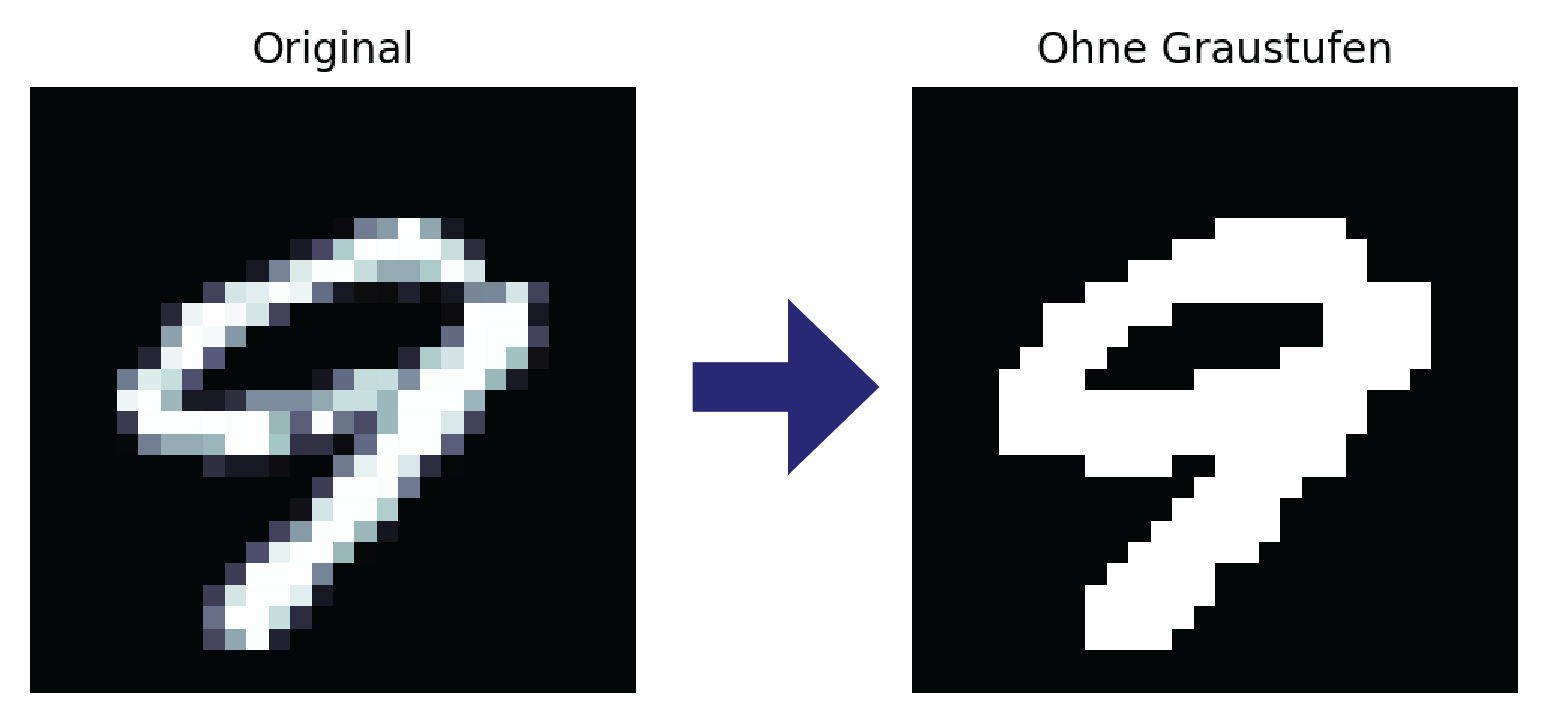
\includegraphics[width=\textwidth]{images/methode/norm-v-nogray.png}
  \caption{Entfernung der Graustufen im MNIST Datenset (eigene Abbildung)}
  \label{fig:norm-v-nogray}
\end{figure}


Das Grundprogramm trainiert mit $3'000$ Bildern, von denen jede Ziffer $300$
Bilder ausmacht. Die restlichen Bilder in den Trainingsdaten sind für mögliche  
Erweiterungen aufgehoben. Der Agent zeichnet jedes der $3'000$ Bilder ein Mal und
trainiert somit für $3'000$ Episodes. Die Der Agent zeichnet für $64$ Steps pro
Episode.

Die Hyperparameter des Grundprogrammes, wie auch die der Variationen (siehe
\doubleref{chap:m_var}) sind durch den Bayesian Optimization Algorithmus
optimiert (siehe \doubleref{sub:t_ml_hyper}). Die Implementierung des
Algorithmus in Python stammt von \cite{fernando_nogueira_bayesian_2014}. Der
Algorithmus ändert sich für verschiedene Variationen der KI nicht und ist somit
Teil des Grundprogrammes. Mit jeder Iteration des Baysian Optimization
Algorithmus trainiert das Reinforcement Learning Modell für eine vom Algorithmus
selbst bestimmte Anzahl Episodes. Die Zielvariable, die durch den Baysian
Optimization Algorithmus maximiert werden soll, wird am Ende jeder Iteration des
Trainings in der Testumgebung berechnet (siehe \doubleref{sub:m_auswert_test}).
Auf welchem der drei Kriterien (siehe \doubleref{chap:m_eval}) die Zielvariable
basiert, ist frei wählbar.



\section{Evaluation der Leistung}\label{chap:m_eval}
In diesem Unterkapitel sind die Kriterien definiert, welche die Leistung der
künstlichen Intelligenz evaluieren. Mit anderen Worten beschreiben die
Kriterien, wie gut die KI nachzeichnet. Für eine präzise und objektive
Evaluation sind alle Kriterien durch einen Zahlenwert repräsentiert. Die
Kriterien und ihre jeweilige Berechnung werden nachfolgend beschrieben.

\subsection{Erkennbarkeit}\label{sub:m_eval_rec}
Das Kriterium der Erkennbarkeit beschreibt, ob in der Vorlage das gleiche Motiv
wie in der Zeichnung der künstlichen Intelligenz erkannt wird. Wenn
Beispielsweise in beiden Fällen eine Fünf erkannt wird, hat das Kriterium den
Wert $1$. Wird in der Vorlage eine Fünf erkannt, aber in der Zeichnung eine
Vier, hat das Kriterium den Wert $0$

Das erkannte Motiv wird durch eine zweite KI beurteilt (siehe
\doubleref{sub:t_ml_func}). Diese zweite KI beurteilt ein Motiv nur als erkannt,
wenn das zugehörige Neuron im Output des neuronalen Netzen einen Wert von über
$0.75$ hat. Das entspricht laut dem neuronalen Netz mit einer hohen
Wahrscheinlichkeit der korrekten Beurteilung.

Um die verschiedenen Arten von Strichbildern, die die KI zeichnen soll, zu
erkennen, existieren vortrainierte Machine Learning Modelle. Die in dieser
Arbeit implementierten vortrainierten Modelle sind in der \autoref{tab:models}
ersichtlich. Diese Modelle sind mit den selben Daten trainiert, die in der
Testumgebung (siehe \doubleref{sub:m_auswert_test}) als Vorlage zum Abzeichnen
dienen.

\begin{table}[!ht]
  \centering
  \begin{tabular}{|l|l|l|l|}
  \hline
      Art & Entwickler & Trainiert mit \\ \hline
      Ziffern & \cite{mazzia__2022} & MNIST \\ \hline
      Buchstaben & \cite{mor_emnist_2022} & EMNIST Letters \\ \hline
      \makecell{Strichbilder\\von Objekten} & \cite{lam_linus_keras_2022} & Auswahl aus QuickDraw \\ \hline
  \end{tabular}
  \caption{Vortrainierte Modelle}
  \label{tab:models}
\end{table}

\subsection{Prozentuale Übereinstimmung}
\label{sub:m_eval_proc}
Dieses Kriterium beschreibt die prozentuale Übereinstimmung der weissen
(gezeichneten) Pixel zwischen der Vorlage und der Zeichnung der KI (siehe
\doubleref{chap:m_grund}). Der Wert $K$ dieses Kriteriums zu dem Step $t$
berechnet sich aus folgender Formel:
\[ K(t) = \frac{G(t)}{G_{\max}} \] $G_{\max}$ entspricht der Anzahl aller
weissen Pixeln in der Vorlage. $G(t)$ entspricht der Anzahl der weissen Pixel,
die zwischen der Vorlage und der Zeichenfläche übereinstimmen. Die Pixel, die
nicht übereinstimmen, zählen negativ für $G(t)$. $G(t)$ und somit auch $K(t)$
können dadurch auch negative Werte annehmen. Der maximale Wert von $K(t)$ ist 1,
was einer prozentualen Übereinstimmung von $100\%$ entspricht (siehe
\autoref{fig:ubereinstimmung}).

%bild übereinstimmung
\begin{figure}[!ht]
  \centering
  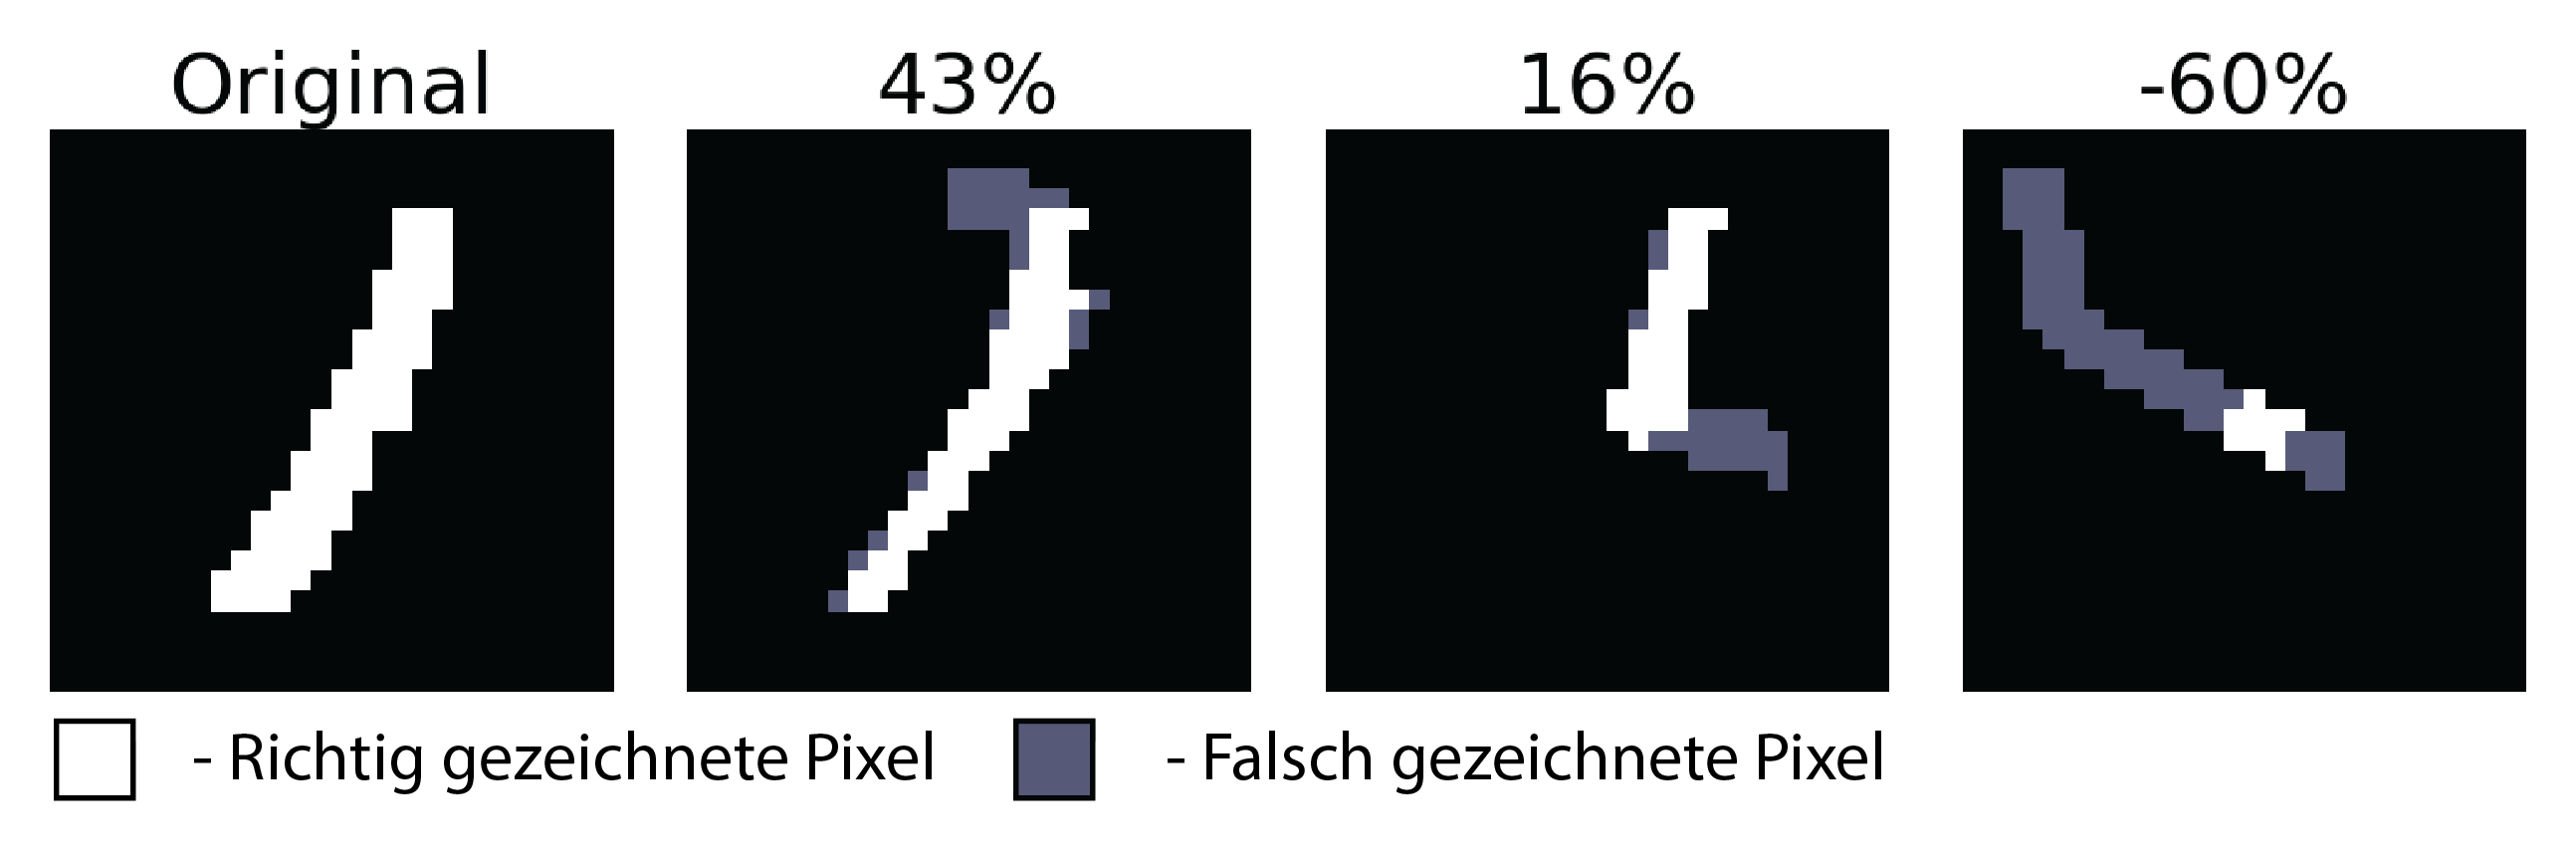
\includegraphics[width=\textwidth]{images/methode/ubereinstimm.png}
  \caption{Drei Beispiele für den Wert des Kriteriums der Übereinstimmung (eigene Abbildung)}
  \label{fig:ubereinstimmung}
\end{figure}

\subsection{Geschwindigkeit}\label{sub:m_eval_speed}
Dieses Kriterium beschreibt, wie schnell die Zeichnung der KI fertig ist. Der
Wert dieses Kriteriums entspricht der Anzahl Steps bis zur Fertigstellung der
Zeichnung. Eine kleinere Anzahl Steps entspricht einer schnelleren Fertigstellung
der Zeichnung und somit einer besseren Leistung bezogen auf dieses Kriterium.

Eine Zeichnung gilt als fertig, wenn die prozentuale Übereinstimmung (siehe
\doubleref{sub:m_eval_proc}) mindestens $70\%$ beträgt und die Zahl der
Definition entsprechend erkannt wird (siehe \doubleref{sub:m_eval_rec}). Wenn
die Zeichnung bis zum Ende der Episode die Bedingungen einer fertigen Zeichnung
nicht erfüllt, hat dieses Kriterium den Wert $64$. Das entspricht der Anzahl
Steps, die von der KI pro Episode insgesamt begangen werden (siehe
\doubleref{sub:m_grund_data}).


\section{Variationen}\label{chap:m_var}
Dieses Unterkapitel beschreibt verschiedene Variationen, ausgehend vom
Grundprogramm (siehe \doubleref{chap:m_grund}). Bei einigen dieser Variationen
handelt es sich um konkrete Implementierungen der definierten Kriterien in die
Reward-Function (siehe \doubleref{sub:t_rl_func}). Die Reward-Function kann
dabei auf mehreren Kriterien gleichzeitig basieren. Der Unterschied zwischen den
Variationen liegt im Fokus auf die Kriterien. Einige Variationen sind
untereinander kombinierbar, andere Variationen führen strukturelle Veränderungen
für die KI ein, die über die Reward-Function hinaus gehen.

\subsection{Basis Reward-Function}\label{sub:m_var_base}
Die Basis Reward-Function ist die einfachste Erweiterung des Grundprogrammes
(siehe \doubleref{chap:m_grund}). Diese Reward-Function implementiert das
Kriterium der prozentualen Übereinstimmung (siehe \doubleref{sub:m_eval_proc}).
Der Reward für eine Action berechnet sich aus der Differenz zwischen der
prozentualen Übereinstimmung vor dem Ausführen der Action, und der prozentualen
Übereinstimmung nach dem Ausführen der Action (also $K(t-1)$ und $K(t)$). Somit
wird der Reward $R$ zum Step $t$ durch folgende Formel berechnet. 
\[ R(t) = K(t) - K(t-1) \] Der Reward eines Steps entspricht folglich nicht der
gesamten prozentualen Übereinstimmung zu einem Step. Stattdessen Entspricht der
Reward der Veränderung der prozentualen Übereinstimmung, ausgelöst durch die
Action in einem Step. Der akkumulierte Reward (siehe \doubleref{sub:t_rl_func})
enstspricht dem absoluten Wert der prozentualen Übereinstimmung.


\subsection{Training auf Geschwindigkeit}\label{sub:m_var_speed}
Das Kriterium der Geschwindigkeit (siehe \doubleref{sub:m_eval_speed}) kann in
die Reward-Function integriert werden. Dadurch trainiert die künstliche
Intelligenz auf eine minimale Zeit bis zur Fertigstellung der Zeichnung. Die
Variation verwendet grundsätzlich die Basis Reward-Function (siehe
\doubleref{sub:m_var_base}). Die vorgeschlagene Anpassung davon sieht
folgendermassen aus: Am Ende jeder Episode wird der Reward jedes Steps in der
Episode mit einem Faktor $f$ multipliziert. Dieser Faktor berechnet sich aus
folgender Formel:
\[ f = 2 - \frac{S}{S_{\max}} \] 
$S_{\max}$ entspricht der Anzahl Steps, die der Agent in einer Episode begeht
(siehe \doubleref{sub:m_grund_data}). $S$ entspricht der Anzahl Steps bis zur
Fertigstellung der Zeichnung. Der Faktor nimmt einen Wert zwischen $1$ und $2$
an. Ein grosser Faktor $f$ entspricht einem hohen Reward und wird durch eine
schnelle Fertigstellung der Zeichnung ausgelöst. Wenn der Agent die Zeichnung
bis zum Ende einer Episode nicht fertigstellt, ist $f = 1$. In diesem Fall unterscheidet sich die
Reward-Function nicht von der Basis Reward-Function. Wenn die Zeichnung früher
fertiggestellt wird, zeichnet der Agent trotzdem alle $S_{\max}$ Steps. Das
verhindert eine ungleichmässige Verteilung zwischen verschiedenen Episodes im
Replay-Buffer (siehe \doubleref{sub:t_rl_func}). In diesem Fall wird $S$
allerdings nur in dem Step gespeichert, in dem die Zeichnung zum ersten Mal die
Bedingung einer Fertigstellung erfüllt.   

Indem das Kriterium der Geschwindigkeit während dem Training angepasst wird,
verstärkt sich der Fokus auf auf eine möglichst schnelle Fertigstellung. Die
minimale prozentuale Übereinstimmung einer fertigen Zeichnung ist als $75\%$
definiert. Zu beginn des Trainings wird dieser Wert auf $25\%$ heruntergesetzt,
und über das Training hinweg linear bis auf $75\%$ erhöht. Dadurch löst die
Reward Function bei einer unfertigen Zeichnung bereits positive Rewards für die
Geschwindigkeit aus. Für diese Anpassung wird Die Bedingung der korrekten
Erkennung (siehe \doubleref{sub:m_eval_speed}) nicht beachtet.


\subsection{Training auf Erkennbarkeit}
\label{sub:m_var_rec}
Das Kriterium der Erkennbarkeit kann, anders als die anderen Kriterien, nur
teilweise in die Reward Function integriert werden. Das Kriterium strebt eine
Erkennbarkeit, unabhängig von der Art der Strichbilder, an (siehe
\doubleref{sub:m_eval_rec}). Die künstliche Intelligenz trainiert allerdings nur
auf das Nachzeichnen von Ziffern. Aus diesem Grund trainiert diese Variation nur
auf die Erkennbarkeit von Ziffern, und lässt die anderen Arten von Strichbildern
aussen vor. 

Die Reward-Function (siehe \doubleref{sub:t_rl_func}) dieser Variation beinhaltet
eine zweite KI, die handgeschriebene Ziffern erkennt (siehe
\autoref{tab:models}). Diese zweite KI beurteilt in jedem Step, welche
Ziffern sie in der Vorlage und in der aktuellen  %TODO Code präzision
Zeichnung erkennt

Die einfachste Form der Reward-Function für diese Variation sähe
folgendermassen aus: Wenn eine Zeichnung das Kriterium der Erkennbarkeit
erfüllt, löst die Reward Function einen Reward von $0.05$. In diesem Zustand
funktioniert die Reward-Function allerdings nicht. Der Agent kann den
akkumulierten Reward nicht maximieren. Zwei Ansätze gehen auf dieses Problem
ein. Beide Ansätze sind Teil dieser Variation.

Der erste Ansatz schlägt vor, die zweite KI erst ab einer gewissen prozentualen
Übereinstimmung (siehe \doubleref{sub:m_eval_proc}) einzusetzen. In diesem Fall
löst die korrekte Erkennung erst ab einer prozentualen Übereinstimmung von
$20\%$ einen positiven Reward aus. Diese zusätzliche Bedingung ist notwendig,
weil die Beurteilungen der zweiten KI teilweise für einen menschlichen
Betrachter fragwürdig sind. Zum Beispiel schätzt die zweite KI eine leere
Zeichenfläche mit einer hohen Sicherheit als eine Eins ein (siehe
\autoref{fig:wrong-minst-rec}). Das ist ein Problem, weil dadurch der Agent
einen positiven Reward für eine leere Zeichenfläche erhält. Das stört das
weitere Lernverhalten, weil es die Wahrscheinlichkeit erhöht, dass die KI nicht
mehr zeichnet.

% Bild falsche mnist rec
\begin{figure}[!ht]
  \centering
  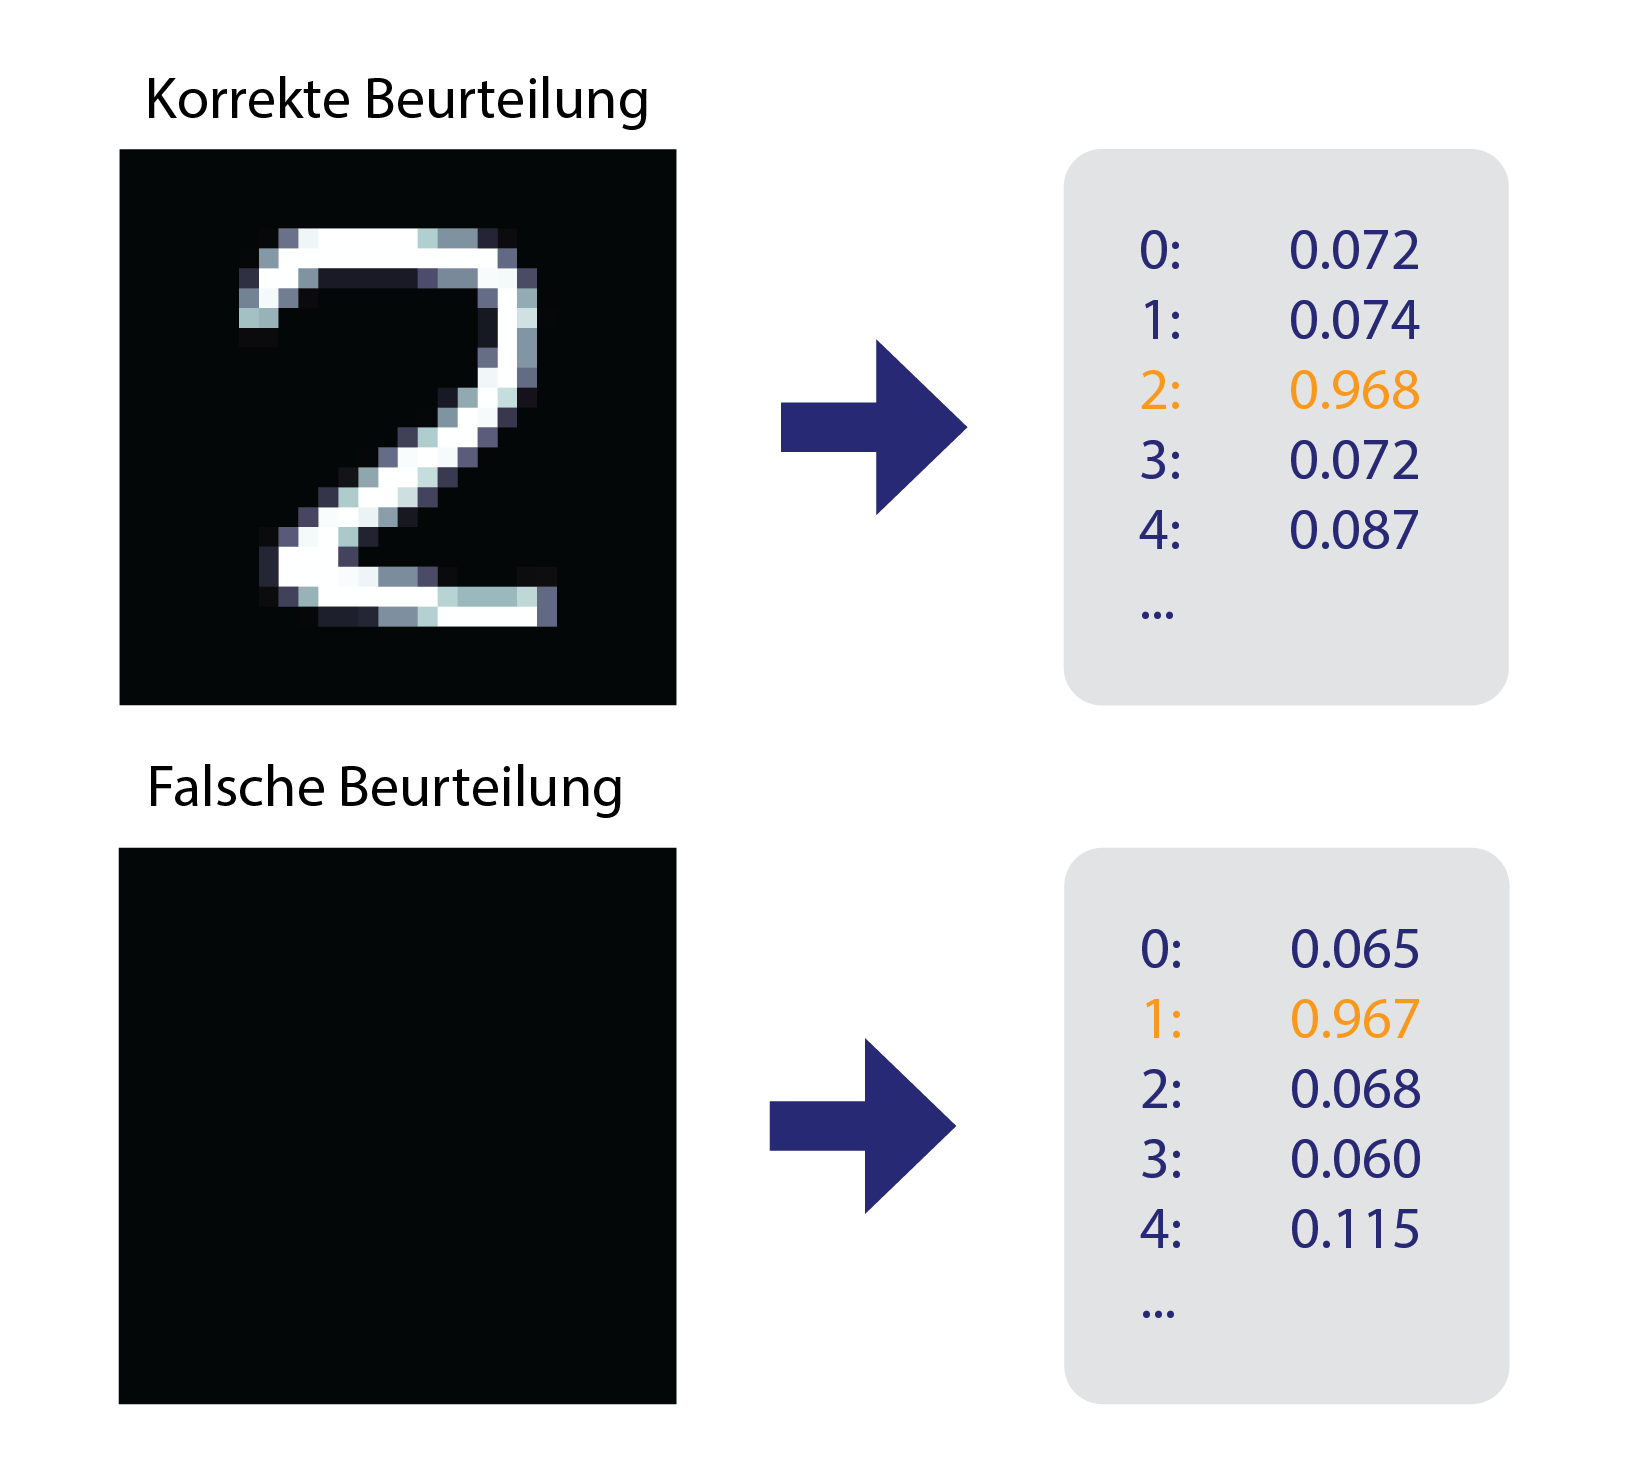
\includegraphics[width=\textwidth]{images/methode/wrong-mnist-rec.png}
  \caption{Beispiele einer richtigen und einer falschen Erkennung von handgeschriebenen Zahlen durch eine KI (eigene Abbildung). Die Werte sind durch einen Test der KI berechnet }
  \label{fig:wrong-minst-rec}
\end{figure}

Der zweite Ansatz implementiert neben der Reward-Function der Erkennbarkeit
erneut die Basis Reward-Function (siehe \doubleref{sub:m_var_base}). Die Relevanz
der beiden Reward-Functions ändert sich allerdings über das Training hinweg. Die
Rewards werden in jedem Step mit einem bestimmten Faktor multipliziert. Zu
Beginn des Trainings ist der Faktor für den Reward der Basis Reward-Function
$f_b = 1$ und der Faktor für den Reward basierend auf der Erkennbarkeit $f_e =
0$. Vom Start ausgehend sinkt $f_b$ linear und $f_e$ steigt linear. Ab einem
gewissen Punkt bleiben beide Faktoren stehen (siehe \autoref{fig:decrementor}).
Blieben die Faktoren ab diesem Punkt nicht konstant, würde die Variation,
gestützt auf Beobachtungen, an der Stabilität ihrer Leistung verlieren.

% Bild Decrementor
\begin{figure}[!ht]
  \centering
  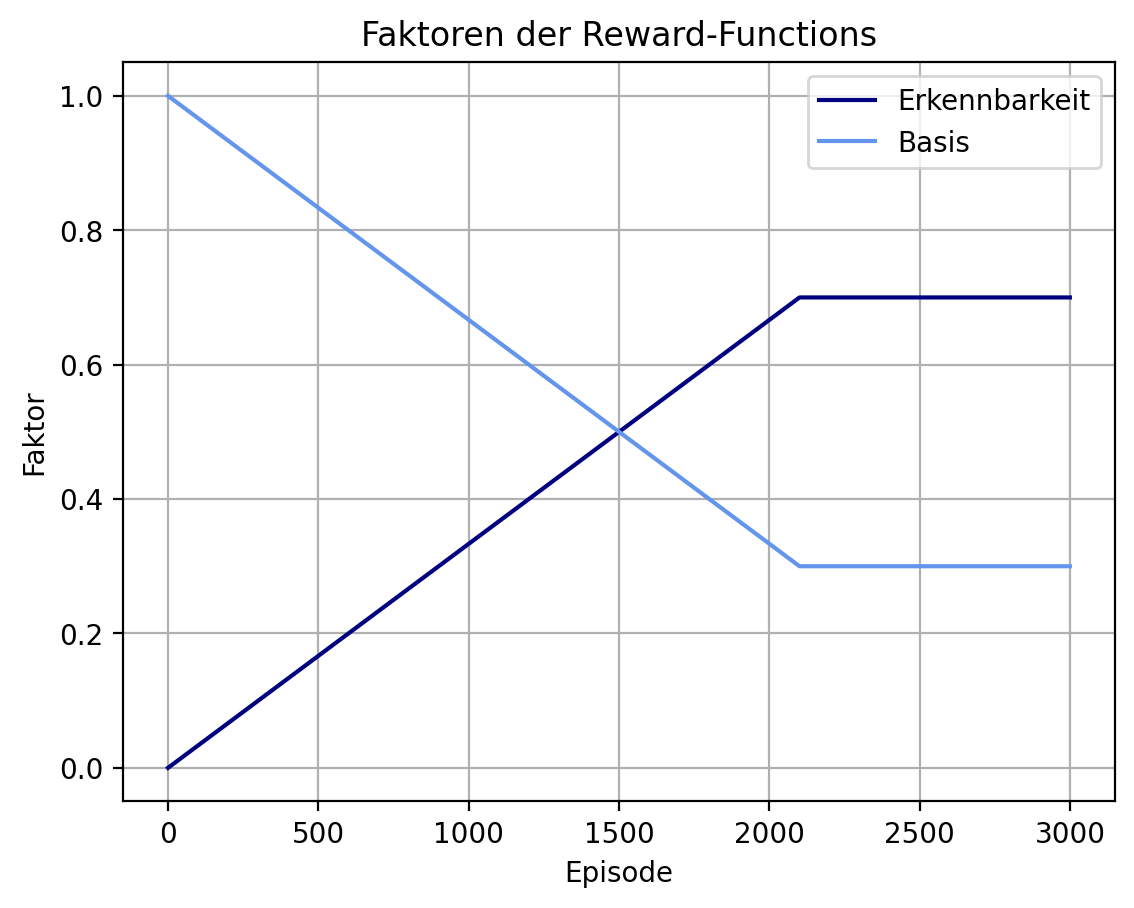
\includegraphics[width=\textwidth-2cm]{images/methode/decrementor.png}
  \caption{Veränderung der Faktoren der Basis Reward-Function und der Reward-Function der Erkennbarkeit über das Training hinweg (eigene Abbildung)}
  \label{fig:decrementor}
\end{figure}

Das Zusammenspiel der beiden Reward-Functions hat den Vorteil, dass die
künstliche Intelligenz zu Beginn des Trainings durch die Basis Reward-Function
für kleine Erfolge positive Rewards erzielt. Die Reward-Function der
Erkennbarkeit ermöglicht das nicht, da sie erst für eine korrekte Erkennung
einen Reward auslöst. Eine Korrekte Erkennung ist allerdings für eine
untrainierte KI schwer zu erreichen. Gewissermassen wird die KI durch die Basis
Reward-Function vortrainiert, um schlussendlich mit der Reward-Function der
Erkennbarkeit effizient trainieren zu können.


\subsection{Physikalische Umgebung}\label{sub:m_var_phy}
Diese Variation spezialisiert sich auf kein Kriterium. Stattdessen verändert
sich die Umgebung, in der sich der Agent bewegt (siehe
\doubleref{sub:t_rl_func}). Auch der Input und der Output des neuronalen Netzes
sind angepasst. Durch diese Veränderungen löst sich die Variation vom
Grundprogramm. Sie bleibt allerdings mit den anderen Variationen kompatibel, Da
diese ausschliesslich die Reward-Function anpassen.

Die Variation ergänzt die Umgebung durch physikalische Simulationen. Diese
physikalische Umgebung definiert die physischen Rahmenbedingungen des Zeichnens
neu, mit dem Ziel, diese näher an die Realität zu bringen.

Der Agent hat neu eine Geschwindigkeit, die durch einen Vektor $\vec{v}$
dargestellt ist. Die Geschwindigkeit beschreibt, um wie viele Pixel und in
welche Richtung sich der Agent pro Step bewegt. Die folgende Formel beschreibt,
wie sich die Position des Agenten vom Step $t$ bis zum nächsten Step $t+1$
ändert:
\[ \vec{p}(t+1) = \vec{p}(t) + \vec{v}(t) \] 
$\vec{p}(t)$ beschreibt die Position des Agents als einen Ortsvektor auf der
Zeichenfläche zum Step $t$ und $\vec{v}(t)$ beschreibt die Geschwindigkeit des
Agenten zum Step $t$. Die Position rundet in jedem Step auf ganze Zahlen. Das
kommt daher, dass die Geschwindigkeit auch Dezimalzahlen annehmen kann, aber die
Position nur durch ganze Zahlen dargestellt ist.

Zur Geschwindigkeit des Agents wird in jedem Step ein Beschleunigungsvektor
addiert. Jede Action, die der Agent wählen kann, entspricht einem anderen
Beschleunigungsvektor. Der Action-Space (siehe \doubleref{sub:t_rl_func})
besteht neu aus $42$ Actions. $21$ der $42$ Actions beschreiben
Beschleunigungsvektoren im zeichnenden Zustand. Die anderen $21$ Actions
beschreiben die selben Vektoren im nicht zeichnenden Zustand. Die 21
verschiedenen Beschleunigungsvektoren im Actions-Space sind in der folgenden
Formation angeordnet: (siehe \autoref{fig:physics-actionspace}). 

%bild physik actionspace
\begin{figure}[!ht]
  \centering
  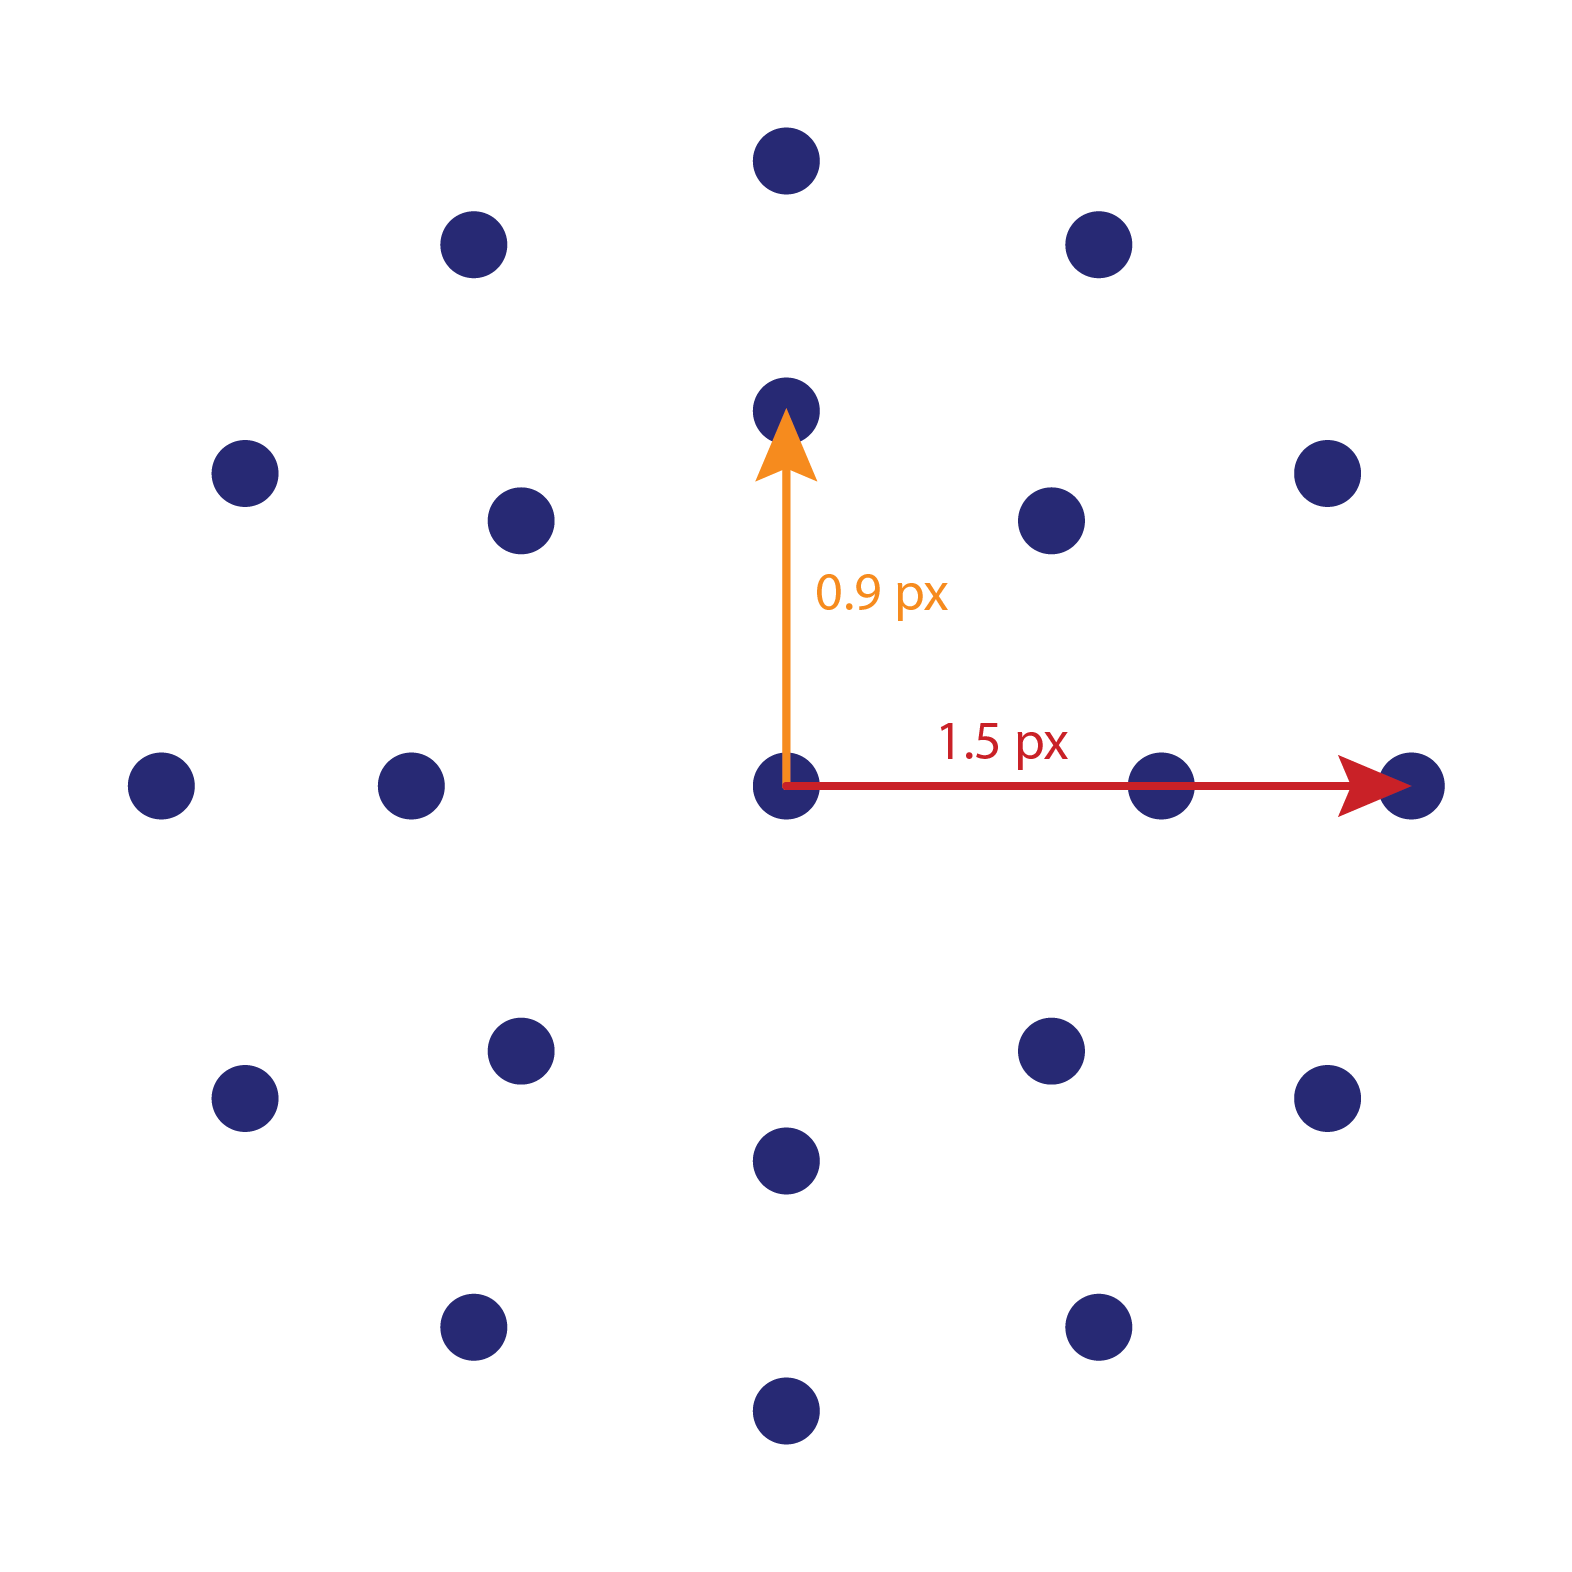
\includegraphics[width=\textwidth-6cm]{images/methode/physics-actionspace.png}
  \caption{Action-Space in der physikalischen Umgebung (eigene Abbildung)}
  \label{fig:physics-actionspace}
\end{figure}


Mit dem gewählten Beschleunigungsvektor $\vec{a}(t)$ berechnet sich die
Geschwindigkeit im nächsten Step $t+1$ aus dem aktuellen Step $t$ durch folgende
Formel:
\[ \vec{v}(t+1) = \vec{v}(t) + \vec{a}(t) \] Der Betrag der Geschwindigkeit
$\vec{v}(t+1)$ des Agents wird in jedem Step, unabhängig von der gewählten
Action, um $0.3$ Pixel pro Step verringert. Das simuliert eine Reibungskraft,
die auf den Agent einwirkt.


Die Veränderungen in der Umgebung erfordern Anpassungen im neuronalen Netz
(siehe \doubleref{sub:t_ml_nn}). Ohne diese Anpassungen kann die KI den
akkumulierten Reward nicht maximieren. Das Problem ist, dass die aktuelle
Geschwindigkeit des Agents kein Teil der Observation ist (siehe
\doubleref{sub:t_rl_func}). Der Agent berücksichtigt deswegen seine
Geschwindigkeit nicht in seinen Entscheidungen. Die Lösung dieses Problems
bietet eine Verschiebung des Local image Patches (siehe \doubleref{sub:t_ver_dood}).
Im Grundprogramm entspricht der Mittelpunkt des Local image Patches genau der
Position des Agents. Neu befindet sich der Mittelpunkt dort, wo sich der Agent
laut seiner aktuellen Geschwindigkeit im nächsten Step befinden wird. Durch
diese Verschiebung des Local image Patches erhält der Agent Informationen über
seine Geschwindigkeit, ohne dessen numerischen Wert zu kennen. Wie im
Grundprogramm gibt der Local image Patch den gesamten Bereich an, in dem sich
der Agent im nächsten Step befinden kann. Die tatsächliche neue Position des
Agents wird durch die Action seiner Wahl bestimmt. Die Grösse des Local image
Patches schrumpft von $7\times7$ Pixeln auf $5\times5$ Pixel, da alle möglichen
Positionen des Agents nach einem Step auf einem $5\times5$ Feld Platz haben
(siehe \autoref{fig:patch-move}). 

%bild local patch verschiebung
\begin{figure}[!ht]
  \centering
  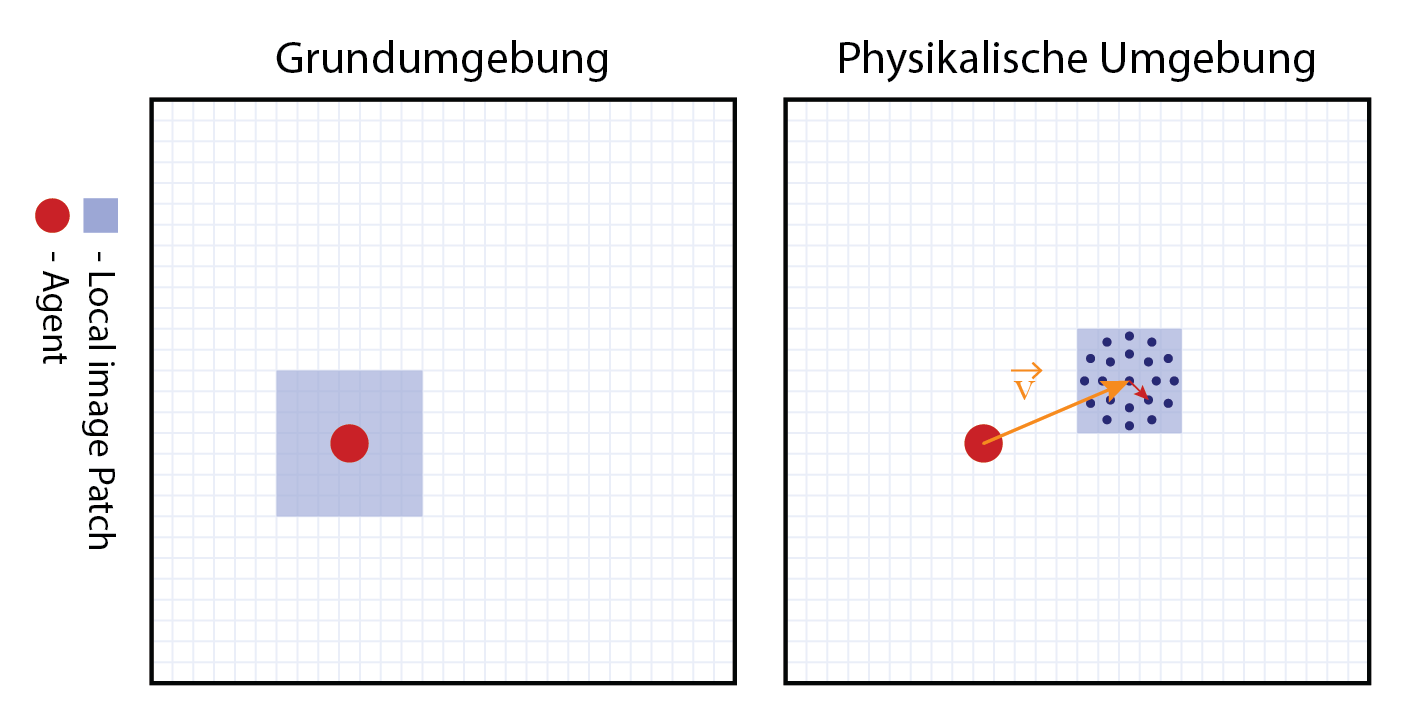
\includegraphics[width=\textwidth]{images/methode/patch-move.png}
  \caption{Angabe der Geschwindigkeit durch eine Verschiebung des Local image Patches (eigene Abbildung)}
  \label{fig:patch-move}
\end{figure}


Ein weiteres Problem ist, dass der Agent sich durch seine Geschwindigkeit aus
den vorgegebenen Grenzen der Zeichenfläche begeben kann. Im Grundprogramm  
(siehe \doubleref{sub:m_grund_dood}) kann der Agent Actions, die ihn in eine
unzulässige Position bewegen würden, nicht auswählen. Wenn allerdings in der
phyiskalischen Umgebung die Geschwindigkeit des Agents zu hoch ist, kann dieser
keine Actions mehr wählen, die ihn innerhalb der Grenzen der Zeichenflächen
halten würden. Als Lösung wird diesen Fällen die Geschwindigkeit des Agents auf den
Nullvektor zurückgesetzt und die Reward Function löst einen negativen Reward von
$-0.05$ aus. Der negative Reward soll die Häufigkeit dieser Vorfälle vermindern.


\section{Auswertung}\label{chap:m_auswert}
Die Auswertung der Daten über die Leistung der künstlichen Intelligenz liefert
das Resultat der Methode. Die Auswertung berechnet den Zahlenwert der
definierten Kriterien (siehe \doubleref{chap:m_eval}) für verschiedene Variationen
der KI.

Die Variationen werden auf ihre Leistung für drei verschiedene Datensets
überprüft. Die drei Datensets beinhalten verschiedene Arten von handgemachten
Strichbildern (siehe \autoref{tab:models}). Das erste Datenset, MNIST,
beeinhaltet Ziffern, die in den Trainingsdaten nicht vorkommen. Das zweite
Datenset, EMNIST Letters, beeinhaltet die 26 Kleinbuchstaben des Alphabets. Das
dritte Datenset, QuickDraw, beeinhaltet Zeichnungen von insgesamt 345
verschiedenen Motiven. Die KI wird allerdings nur auf das Nachzeichnen von zehn
Motiven überprüft. Die zehn Motive sind: `Amboss', `Apfel', `Besen', `Eimer',
`Bulldozer', `Uhr', `Wolke', `Computer', `Auge' und `Blume' (siehe
\autoref{fig:quickdraw-examples}). Die Bilder in den
drei Datensets sind gleich verarbeitet wie die Trainingsdaten (siehe
\doubleref{sub:m_grund_data}). 

%Bild images dataset
\begin{figure}[!ht]
  \centering
  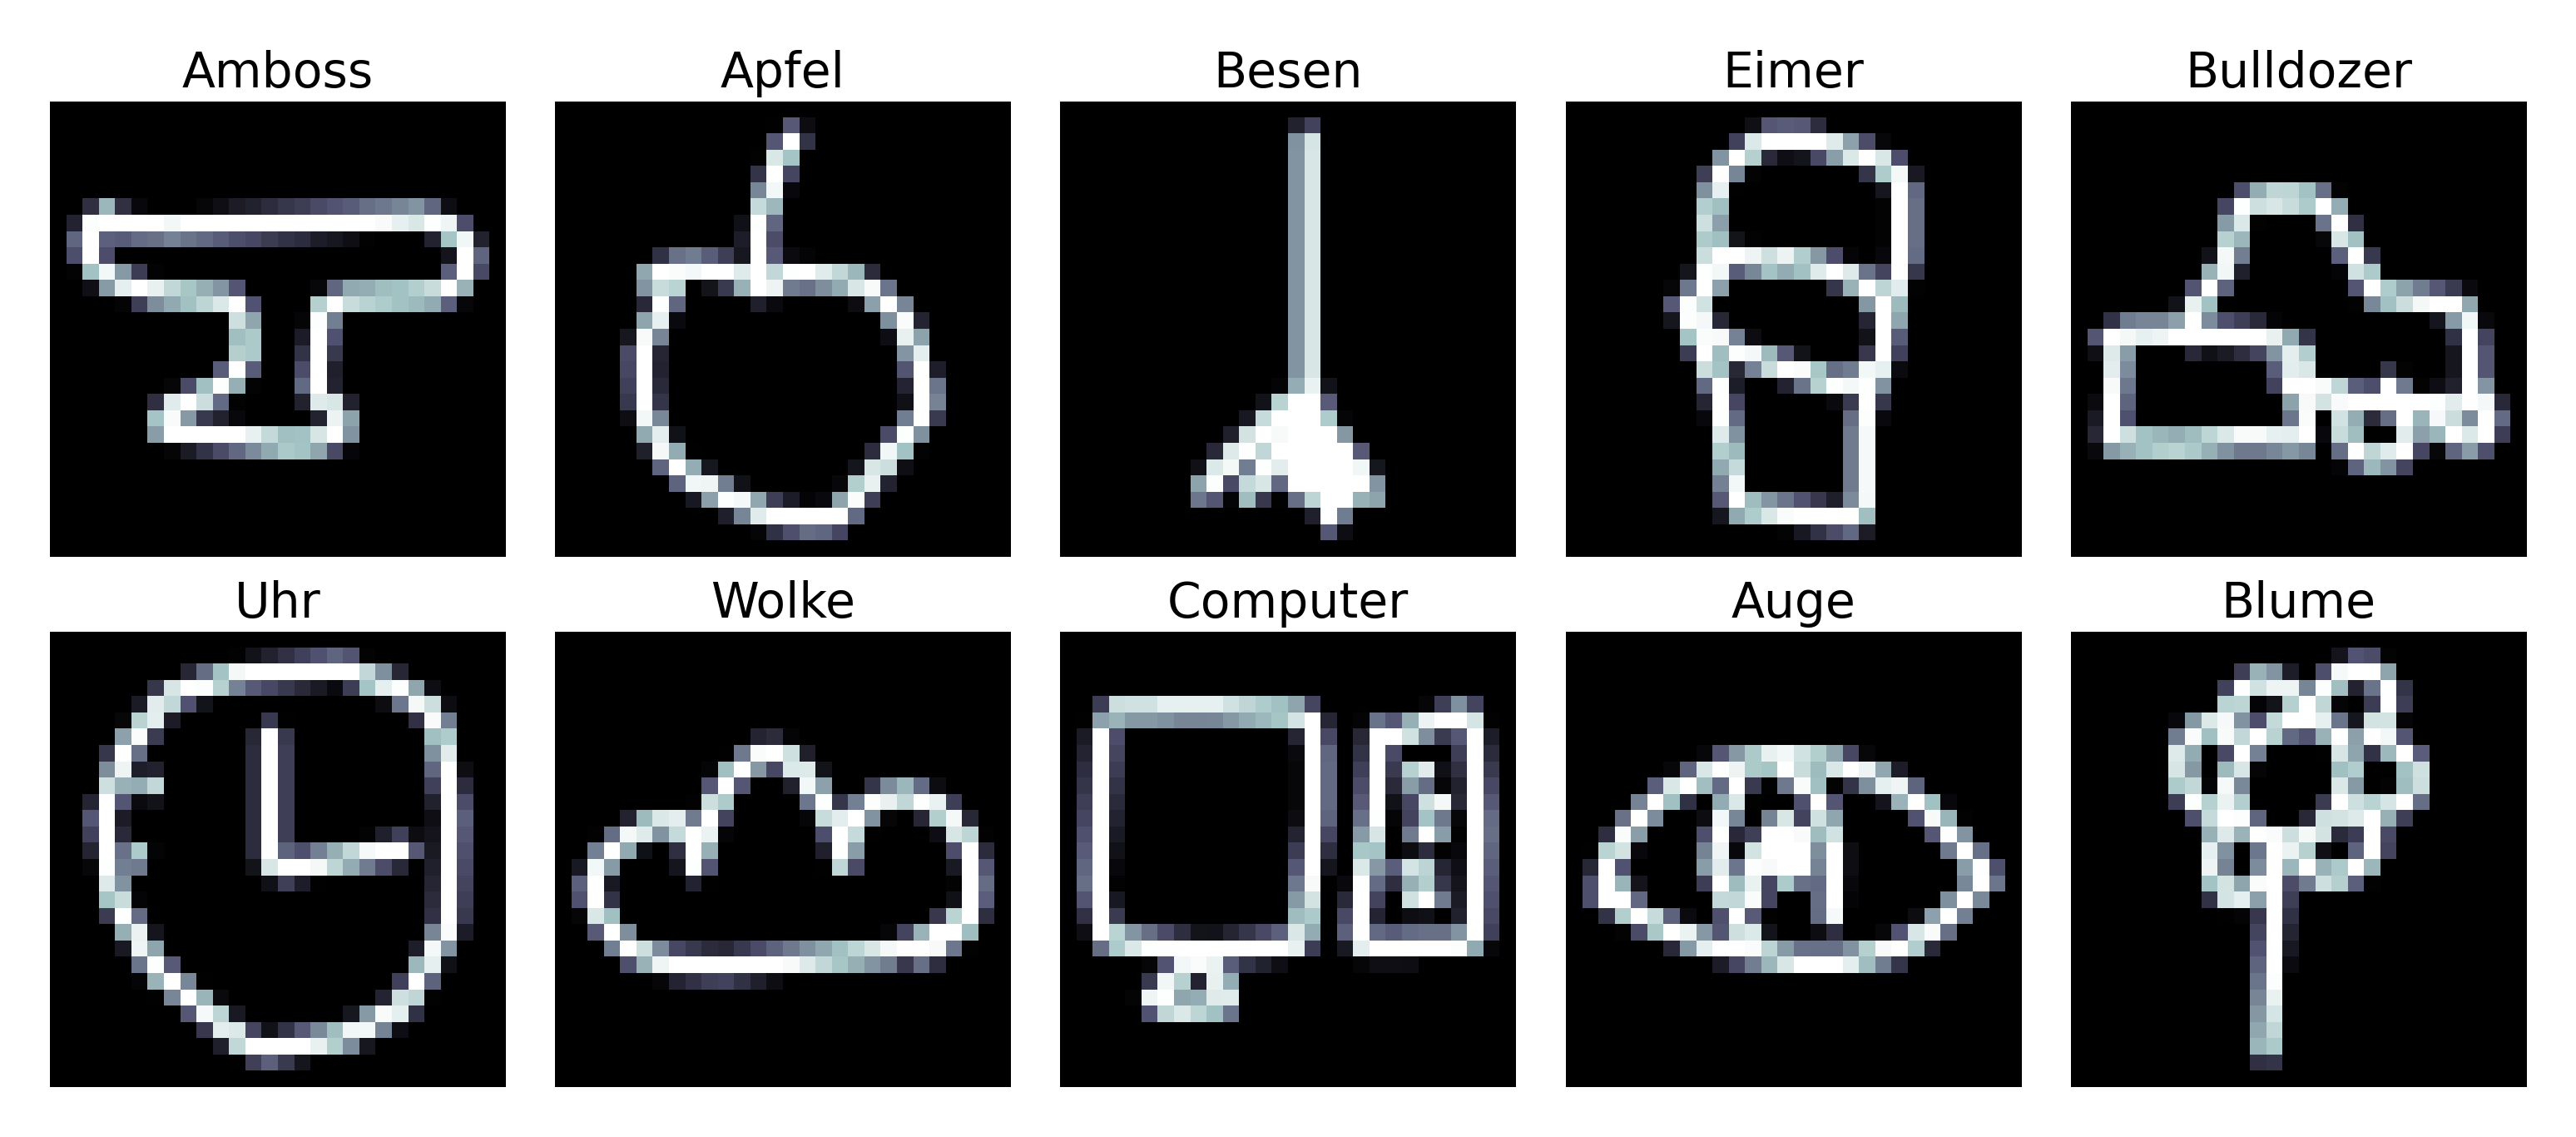
\includegraphics[width=\textwidth]{images/methode/quickdraw-examples.png}
  \caption{Beispiele der verwendeten Motiven aus dem QuickDraw Datenset}
  \label{fig:quickdraw-examples}
\end{figure}


Die Variationen (siehe \doubleref{chap:m_var}) der KI umfassen zwei Umgebungen und
drei Reward-Functions \doubleref{sub:t_rl_func}. Für jede Variation ist zur
Vereinfachung eine Abkürzung definiert.
\begin{itemize}
  \item \doubleref{chap:m_grund} Umgebung: Grund
  \item \doubleref{sub:m_var_phy}: Physik
  \item \doubleref{sub:m_var_rec}: Basis
  \item \doubleref{sub:m_var_speed}: Speed
  \item \doubleref{sub:m_var_rec} (von MNIST Ziffern): MNIST
\end{itemize}

Die folgenden Kombinationen an Variationen der künstlichen Intelligenz werden
ausgewertet. Diese Kombinationen stellen einzelne Versionen der KI dar
\begin{itemize}
  \item Grund-Basis
  \item Grund-MNIST
  \item Grund-Speed
  \item Grund-MNIST-Speed 
  \item Physik-Basis
  \item Physik-MNIST
  \item Physik-Speed
  \item Physik-MNIST-Speed
\end{itemize}

\subsection{Testumgebung}\label{sub:m_auswert_test}
Die Leistungen der verschiedenen Variationen der künstlichen Intelligenz werden
in einer Testumgebung (siehe \doubleref{sub:t_ml_func}) ausgewertet. Zwischen der
Trainingsumgebung und der Testumgebung sind drei relevante Unterschiede
erkennbar. Erstens trainiert die KI in der Testumgebung nicht. Die Testumgebung
übernimmt eine trainierte Version der KI und verändert diese während dem Test
nicht. Zweitens wählt der Agent in keinem Fall mehr eine zufällige Action.
Stattdessen wählt er immer die Action mit dem höchsten Q-Value (gleichbedeutend
mit $\epsilon = 0$) (siehe \doubleref{sub:t_rl_func}). Der Dritte Unterschied
liegt in den Strichbildern, die für die künstliche Intelligenz als Vorlage
dienen. Im Test zeichnet das Computerprogramm $2000$ Bilder aus einem der drei
zur Verfügung stehenden Datensets (siehe \autoref{tab:models}). 

Am Ende jeder Episode (das heisst jeder Zeichnung), wird der Zahlenwert für die
verschiedenen Kriterien (siehe \doubleref{chap:m_eval}) nach ihrer Definition
ausgewertet und gespeichert. Die KI zeichnet auch in der Testumgebung für $64$
Steps. Wenn eine Zeichnung der Definition entsprechend früher fertig ist (siehe
\doubleref{sub:m_eval_speed}), wird die Anzahl Steps zu diesem Zeitpunkt als Wert
des Kriteriums der Geschwindigkeit gespeichert und die KI zeichnet weiter. Der
Durchschnitt aller gespeicherten Werte eines Kriteriums entspricht der Leistung
der getesteten Variation in diesem Kriterium. Das Kriterium der Erkennbarkeit
(siehe \doubleref{sub:m_eval_rec}) verwendet zur Auswertung entsprechend dem
verwendeten Datenset im Test, dasjenige vortrainierte Modell, das auf dem selben
Datenset trainiert ist. Da das Kriterium der Erkennbarkeit jeweils den Wert $0$
oder $1$ hat, ergibt der Durchschnitt aus allen Werten dieses Kriteriums eine
prozentuale Angabe (in Dezimalform) darüber, in wie vielen Fällen das richtige
Motiv erkannt wird.



